% % % % % % % % % % % % % % % % % % % % % % % % % % % % % % % % % % % % 
% 
% FS-Vorlage											Stand: 30.01.12
%
% Formelsammlungsvorlage von Emanuel Regnath und Martin Zellner	
% Bietet verschiedene Abkürzungen und Befehle	
%
% % % % % % % % % % % % % % % % % % % % % % % % % % % % % % % % % % % % 


% Dokumenteinstellungen
% ======================================================================

% Dokumentklasse (Schriftgröße 6, DIN A4, Artikel)
\documentclass[6pt,a4paper]{scrartcl}


% Pakete laden
\usepackage[utf8]{inputenc}		% Zeichenkodierung: UTF-8 (für Umlaute)   
\usepackage[german]{babel}		% Deutsche Sprache
\usepackage{amsmath}			% erlaubt mathematische Formeln
\usepackage{amssymb}			% Verschiedene Symbole
\usepackage{esint}				% erweiterte Integralsymbole
\usepackage{multicol}			% ermöglicht Seitenspalten  
\usepackage{booktabs}			% bessere Tabellenlinien
\usepackage{graphicx}			% Zum Bilder einfügen benötigt
\usepackage{pbox}				%Intelligent parbox: \pbox{maximum width}{blabalbalb \\ blabal}
\usepackage{accents}			% Für eigene Ableitungspunkte benötigt
% \usepackage{undertilde}		wozu brauchen wir das?
\usepackage{scrtime}


% .:: Seitenlayout und Ränder
% ======================================================================
\usepackage{geometry}
\geometry{a4paper,landscape, left=6mm,right=6mm, top=0mm, bottom=3mm,includeheadfoot} 


% .:: Kopf- und Fußzeile
% ======================================================================
\usepackage{fancyhdr}
\pagestyle{fancy}
\fancyhf{}

   \fancyfoot[C]{von Max Mustermann}
   \renewcommand{\headrulewidth}{0.0pt} %obere Linie ausblenden
   \renewcommand{\footrulewidth}{0.1pt} %obere Linie ausblenden

   %\fancyfoot[R]{Stand: \todayV \ um \thistime \ Uhr \qquad \thepage}
   \fancyfoot[L]{Homepage: emareg.de - Fehler bitte sofort melden.}
	
% Schriftart SANS für bessere Lesbarkeit bei kleiner Schrift
\renewcommand{\familydefault}{\sfdefault} 
% Array- und Tabellenabstände vergrößern
\renewcommand{\arraystretch}{1.2}

% Eigene Befehle
\newcommand{\iset}[2]{\ensuremath{\bigl\{ \bigl. #1 \, \bigr| \, #2 \bigr\}}}	%intensional set
\newcommand{\eset}[1]{\ensuremath{\bigl\{#1\bigr\}}}							%extensional set
\newcommand{\enbrace}[1]{\ensuremath{\bigl\(#1\bigr\)}}							%große Klammern
\newcommand{\norm}[1]{\ensuremath{\|#1\|}}										%Norm
\newcommand{\abs}[1]{\ensuremath{\left\vert#1\right\vert}} 						%Betrag
\newcommand{\mat}[1]{\ensuremath{\begin{bmatrix} #1 \end{bmatrix}}}				%Matrix
\newcommand{\ma}[1]{\ensuremath{\utilde{\boldsymbol {#1}}}}						%Matrixsymbol
\newcommand{\vect}[1]{\ensuremath{\begin{pmatrix} #1 \end{pmatrix}}}			%Vektor
\newcommand{\mvect}[1]{\ensuremath{\left. \begin{matrix} #1 \end{matrix}  \right]}} %Matrixvektor
\newcommand{\gk}[1]{\ensuremath{\left\lfloor#1\right\rfloor}} 					%Gaußklammer
\newcommand{\sprod}[2]{\ensuremath{\left\langle #1, #2 \right\rangle }}			%Skalarprodukt
\newcommand{\bdot}{\ensuremath{\boldsymbol \cdot}} 								%Dicker Punkt für Skalarprodukt


% Befehle sichern
\let\oldvec = \vec
\let\olddot = \dot

% Überschreibungen
\renewcommand{\vec}[1]{\ensuremath{\underline{\boldsymbol {#1}}}}
\renewcommand{\emph}[1]{\textbf{#1}}
\renewcommand*{\dot}[1]{\accentset{\mbox{\textrm{\large\bfseries .}} }{#1}}
\renewcommand*{\ddot}[1]{\accentset{\mbox{\textrm{\large\bfseries .\hspace{-0.25ex}.}}}{#1}}
\renewcommand{\i}{\ensuremath{\mathrm{j}}}										%imaginäre Einheit

% Abkürzungen
\newcommand{\ul}[1]{\ensuremath{\underline{#1}}}								%Untersteichen
\newcommand{\ol}[1]{\ensuremath{\overline{#1}}}									%Überstreichen
\newcommand{\Ra}[0]{\ensuremath{\Rightarrow}}									%Rightarrow
\newcommand{\ra}[0]{\ensuremath{\rightarrow}} 									%Rightarrow
\newcommand{\bs}[1]{\ensuremath{\boldsymbol{#1}}}								%Fett und kursiv im mathmode
\newcommand{\diff}{\ensuremath{\ \mathrm d}}									%delta
\newcommand{\grad}{\ensuremath{\mathrm{grad}\,}}								%Gradient
\renewcommand{\div}{\ensuremath{\mathrm{div}\,}}								%Divergenz
\newcommand{\rot}{\ensuremath{\mathrm{rot}\,}}									%Rotation
\newcommand{\Sp}{\ensuremath{\mathrm{Sp}\,}}									%Spur
\newcommand{\ggT}{\ensuremath{\mathrm{ggT\,}}}									%ggT
\newcommand{\e}{e}																%Eulersche Zahl
	% Für Mengen
	\newcommand{\N}{\ensuremath{\mathbb N}}
	\newcommand{\R}{\ensuremath{\mathbb R}}
	\newcommand{\C}{\ensuremath{\mathbb C}}
	\newcommand{\Z}{\ensuremath{\mathbb Z}}
	\newcommand{\K}{\ensuremath{\mathbb K}}
	


% Dokumentbeginn
% ======================================================================
\begin{document}


% Aufteilung in Spalten
\begin{multicols}{4}

% ---------------------------------------
% | 		Energietechnik	 			|
% ~~~~~~~~~~~~~~~~~~~~~~~~~~~~~~~~~~~~~~~
%=======================================================================

	\section{Physikalische Grundlagen}
	$P = M \cdot \omega$ \\
	$\omega = 2 \pi n$

	\section{Lastganglinien}
	$T_n$: Nennbetriebsdauer\\
	$T_a$ Ausnutzungsadauer\\
	$T_{ben}$: Benutzungsdauer\\
	$P_{max}$: Höchstalast\\
	$W = \int_0^{T_n} P(t) \diff t = P_{mittel} T_n = P_n T_a = P_{max} T_{ben}$\\
	
	\section{Wechel-/Drehstromsystem}


		\subsection{Wechselstromsystem}
		Phasenwinkel $\varphi = \varphi_u - \varphi_i$ \qquad Kreisfrequenz: $\omega = 2\pi f$\\
		
		
		Physikalische Zeitsignale:\\
		$u(t) = \hat u \cos(\omega t + \varphi_u) = U \sqrt{2} \cos(\omega t + \varphi_u)$\\
		$i(t) = \hat i \cos(\omega t + \varphi_i) = I \sqrt{2} \cos(\omega t + \varphi_i)$\\
		\\
		Komplexes Zeitsignal(Drehzeiger): $\vec u(t) = \hat u \exp\big(\i (\omega t + \varphi_u)\big)$, 
		$u(t) = \Re(\vec u(t))$\\
		
	
		Scheitelwert $\hat u$, Effektivwert $U = \sqrt{\frac{1}{T} \int_{t_0}^{t_0 + T} u^2(\tau) \diff \tau}$,
		bei Sinus $U = \frac{\hat u}{\sqrt{2}}$\\
		Effektiver Zeiger: $\vec U = U \exp(\i \varphi_u)$\\
		
		$\vec U \cdot \sqrt{2} \exp(\i \omega t) = \vec u(t)$	
	

	
		\subsection{Komplexe Leistung}
		$P = \frac1T \int_0^{T} p(t) \diff t = \frac1T \int_0^{T} u(t) \cdot i(t) \diff t$\\
		\begin{tabular}{lll}
		Wirkleistung & $P = \Re(\vec S) = U I \cdot \cos(\varphi)$ & [W] \\
		Blindleistung & $Q = \Im(\vec S) = U I \cdot \sin(\varphi)$ & [Var]\\
		Scheinleistung & $S = U \cdot I = \sqrt{P^2 + Q^2}$ & [VA]\\
		\end{tabular}
		\pbox{8.0cm}{
		Scheinleistung: $\vec S = \vec U \cdot \vec I^*$ \\ $\norm{\vec S} = S = \sqrt{P^2 + Q^2}$\\ Leistungsfaktor $\lambda = \frac{|P|}{S} = \cos(\varphi)$ } \qquad
		\pbox{4cm}{ 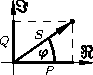
\includegraphics{./img/leistung.pdf} }\\
		
		Scheinleistung schwingt mit doppelter Netzfrequenz!
		$p(t) = P + S \cdot \cos(2\omega t + \varphi_u + \varphi_i)$\\
		$\tilde {\vec S} = \vec U \cdot \vec I$\\

		\begin{tabular}{ll}
		Impedanz(Scheinwiderstand) & Admittanz(Scheinleitwert)\\
		$\vec Z = R + \i X = \exp(\i \varphi_Z)$ & $\vec Y = G + \i B = \exp(\i \varphi_Y)$\\
		$\underset{\text{Impedanz}}{Z(j\omega)} = \underset{\text{Resistanz}}{R(j\omega)} + \underset{\text{Reaktanz}}{jX(j\omega)}$ & 	$\underset{\text{Admittanz}}{Y(j\omega)} = \underset{\text{Konduktanz}}{G(j\omega)} + \underset{\text{Suszeptanz}}{jB(j\omega)}$\\
		$\vec U = \vec Z \cdot I $ & $\vec I = \vec Y \cdot \vec U$\\

		\end{tabular}



		\subsection{Drehstromsystem}
		Drehoperator: $\vec a = \exp\bigl(\i \frac{2}{3} \pi \bigr)$ \qquad $\vec a^0 = \vec a^3 = 1$ \quad $\vec a^* = \vec a^2$\\
		
		% Zeigerdiagramm mit Drehoperatoren
		
		Effektive Leiter-Erdspannungen: $\vec U_1,\vec U_2,\vec U_3$\\
		Effektive Außenleiterspannungen: $\vec U_{12},\vec U_{23},\vec U_{31}$\\
		symmetrischer Betrieb:\\
		$U = |U_1| = |U_2| = |U_3|$\\
		Netznennspannung: $U_n = |U_{12}| = |U_{23}| = |U_{32}| = \sqrt{3} U$\\
		Gesamte Leistung: $\vec S = \sqrt{3} \cdot \vec U_n \cdot \vec I^\star$\\
		bei symmetrischem Betrieb: $\vec S = 3 \cdot \vec U \cdot \vec I$\\
		bei unsymmetrischem Betrieb: 
		\[\vec S = \vec U_1 \cdot \vec I_1^\star + \vec U_2 \cdot \vec I_2^\star + \vec U_3 \cdot \vec I_3^\star\]
		
		Komplexe Wechselleistung:
		\[\tilde{\vec S} = \vec U_1 \cdot \vec I_1 + \vec U_2 \cdot \vec I_2 + \vec U_3 \cdot \vec I_3\]
		Tatsächlicher Leistungsfluss:
		\[p(t) = \operatorname{Re} \left\{ \vec S \right\} + \operatorname{Re} \left\{\tilde{\vec S} e^{j 2 \omega t} \right\}\]
		
	\section{Elektrische Energieübertragung}
	
		\subsection{Drehstromleitung}
		
		% einphasiges ESB für den symmetrischen Betrieb
		
		\[\begin{pmatrix} \vec U_1 \\ \vec U_2 \\ \vec U_3 \end{pmatrix} = \begin{pmatrix} \vec Z_d & \vec Z_k & \vec Z_k \\ \vec Z_k & \vec Z_d & \vec Z_k \\ \vec Z_k & \vec Z_k & \vec Z_d \end{pmatrix} \begin{pmatrix} \vec I_1 \\ \vec I_2 \\ \vec I_3 \end{pmatrix}\]
		Im symmetrischen Betrieb kann im einphasigen ESB $Z_b$ als Leitungsimpedanz eingesetzt werden: $\vec Z_b = \vec Z_d - \vec Z_k$


	\section{Elektrische Maschinen}
	können als Motoren oder Generatoren benutzt werden. ($\eta > 90\%$)\\
	Besteht aus Stator(Ständer),Rotor(Läufer), Anker und Welle.\\
	$n:$ Drehzahl; $M:$ magn. Moment\\


		\subsection{Der Transformator}
		\begin{tabular}{cl}
		ü & Übersetzung \\
		$"u_r$ & Bemessungsübersetzung \\
		$U_{r1T}$, $U_{r2T}$ & Bemessungsspannungen \\
		$S_{rT}$ & Bemessungsleistung \\
		$U_{K}$ & Kurzschlussspannung \\
		$u_k$ & bezogene Kurzschlussspannung \\
		$u_r$ & bezogener Wirkspannungsabfall \\
		$P_{Cu}$ & Kupferverluste \\
		$P_{Fe}$ & Eisenverluste \\
		$Z_k$ & Kurzschlussimpedanz
		\end{tabular}
		
		% Ersatzschaltbild

		Zur Berechnung wird oft $"u_r$ anstelle von $"u$ eingesetzt, da ersteres meist unbekannt ist. Die Bemessungsübersetzung findet sich aber auf dem Typenschild. \\
		$\vec U^b = "u \vec U$ \\
		$\vec I^b = \frac{1}{"u} \vec I$ \\
		$\vec Z^b = "u^2 \vec Z$ \\
		$"u = \frac{W_1}{W_2}$ \\
		$"u_r = \frac{U_{r1T}}{U_{r2T}}$ \\
		$u_k = \frac{U_{K}}{U_{r1T}}$ \\
		$Z_k = u_k \frac{U_{r1T}^2}{S_{rT}}$ \\
		$u_r = \frac{U_{rT}}{U_{r1T}}$ \\
		$R_k = P_{Cu} \left( \frac{U_{r1T}}{S_{rT}} \right)^2$ \\
		$R_k = u_r \frac{U_{r1T}^2}{S_{rT}}$ \\
		$Z_k = \sqrt{R_k^2 + X_k^2}$ \\
		$R_{Fe} = \frac{U_{r1T}^2}{P_{Fe}}$ \\
		$I_{W0} = \frac{P_{Fe}}{\sqrt{3} U_{r1T}}$ \\
		$I_h = \sqrt{I_{10}^2 - I_{W0}^2}$ \\
		$X_h = \frac{U_{r1T}}{\sqrt{3} I_h}$
	
		\subsection{Gleichstrommaschine}
		
		\begin{tabular}{cl}
		$p$ & Polpaarzahl \\
		$z$ & Anzahl der Schaltstufen \\
		$\lambda$ & Schaltverhältnis \\
		$U$ & Ankerklemmenspannung \\
		$U_i$ & Im Anker induzierte Spannung \\
		$K_1$, $K_2$ & Maschinenkonstanten \\
		$\Phi$ & magnetischer Fluss durch den Anker \\
		$I_A$ & Ankerstrom \\
		$R_A$ & Widerstand der Ankerwicklungen \\
		$I_E$ & Erregerstrom
		\end{tabular}
		
		\subsubsection{Grundgleichungen}
		$U = U_i + (R_A + R_v) I_A = U_i + RI$\\
		$U_i = K_1 \Phi n$\\
		$M = K_2 \Phi I_A$\\
		$\Phi = f(I_E)$\\
		falls verlustfrei: $K_1 = 2 \pi K_2$ \\
		$n = \frac{U}{ K_1 \cdot \Phi} - \frac{R}{K_1 \cdot K_2 \cdot \phi^2}M$\\
		
		% Ersatzschaltbild
		
		\subsubsection{Anlaufen mit Vorwiderständen}
		$R_{A_,z-1} = R_A + R_{V1}$, $R_{A_,z-1} = R_A + R_{V1} + R_{V2}$, ..., $R_{A,0} = R_A + R_{V1} + \hdots + R_{Vz}$ \\
		$\lambda = \frac{M_{max}}{M_{min}} = \frac{R_{A,Z-1}}{R_{A,Z}}$ \\
		$ z = \log_\lambda \frac{R_{A0}}{R_A}$
		
		% Bild der Vorwiderstände
		
		\subsubsection{Fremderregt}
		$n_0 = \frac{U}{K_1 \Phi}$ \\
		$M_A = \frac{U K_2 \Phi}{R}$ \\
		$n = n_0 - n_0 \frac{M}{M_A}$
		
		% Ersatzschaltbild
		
		\subsubsection{Reihenschluss}
		$M = \frac{K_2}{K_3} \Phi^2$ \\
		$n = \frac{U}{\sqrt{2 \pi K_1 K_2}} \frac{1}{\sqrt{M}} - \frac{R}{K_1 K_2}$
		
		% Ersatzschaltbild
		
		\subsection{Synchronmaschine}
		
		% Ersatzschaltbild
		
		Synchrone Reaktanz $X_d = \omega \cdot (L_h + L_\sigma)$\\
		$X_d \cdot I_w = U_p \sin(\vartheta_M)$\\
		$X_d = x_d \frac{U_r^2}{S_r}$ \\
		\begin{tabular}{ll}
			Übereregung & Untereregung\\ \midrule
			SMA wirkt wie Kapazität & SMA wirkt wie Induktivität\\
			gibt induktive Blindleistung ab & nimmt induktive Blindleistung auf\\
		\end{tabular}
		
		\subsection{Asynchronmaschine}
		Bemessungsmoment $M_r = \frac{P_r}{2\pi n_r}$\\
		Kloss'sche Gleichung $M = \frac{2 M_k \cdot s \cdot s_k}{s^2 + s_k^2}$
		
		Kippmoment $M_k$; Betrieb bei ca. $\frac{2}{3} M_k \Rightarrow \vartheta_M < 42^\circ$\\
		
		\subsection{Asynchronmaschine}
		 
		 % Ersatzschaltbild
		 
		 $s = \frac{n_0 - n}{n_0}$ \\
		 $M = \frac{3}{2 \pi n_0} \frac{I^2 R_l}{s}$ \\
		 $n_0 = \frac{f}{p}$ \\
		 $M = \frac{2 M_k}{\frac{s}{s_k} + \frac{s_k}{s}}$


		Anlauf nur möglich falls $M_A < M_{an}$\\

		Feldschwächung: $\Phi_M \propto \frac{U_{st,r}}{f_{st,r}}$\\
		$U$ kann nicht beliebig erhöht werden $\Ra$ Fluss wird kleiner $\Ra$ Moment wird kleiner.\\
		
		
		
	\subsection{elektrische Energieübertragung}
	Freileiter oder Erdleiter:\\
	\begin{itemize}
		\item Erdkabel-Isolierung: Papier mit Öl getränkt oder vernetztes PE
		\item Erdakabel bei gleicher Übertragung etwa 4 -- 7 mal teuerer.
		\item Störungen bei Freileitern leichter lokalisierbar und behebbar.\\
	\end{itemize}
	Längsimpedanzen (KS) und Queradmittanzen (LL)

	\begin{tabular}{llllll}
		$U_n$ & Leitung & Leiter & $R$ & $X'_b = \omega L'_b$ & $Y_b = \omega C'_b$ \\
		30kV & FL & Al/St 95/15 & 0.30 & 0.37 & \\
	\end{tabular}

	$\vec U_{12} = \Delta U + \i \delta U$\\
	meist $R << \omega L_b$ \quad $\Ra \vec U_{12} = \omega L_b (I_w + I_b)$\\

	Phasenkonstante $\beta = 2 \pi f \frac{\sqrt{\varepsilon_r}}{c_0}$ \qquad $\beta(FL) \approx \frac{6^\circ}{100km}$\\
	
	\begin{tabular}{lll}
	& $\vec Z_l$ & $\frac{\vec Y_q}{2}$\\[0.5em] \midrule
	el. lange Leitung & $\i \vec Z_w \sin(\beta l)$ & $\frac{\cos(\beta l) -1}{\i \vec Z_w \sin(\beta l)}$\\[0.5em]
	el. kurze Leitung & $\i \omega L'_b I$ & $\frac{\i \omega C'_b l}{2}$\\[0.5em]
	\end{tabular}

	natürlicher Betrieb( $\vec Z_2 = \vec Z_w$ ): Blindleistungsggw\\


	\subsection{Vereinfachte Leitungsbetrachtung}
	Vernachlässigung von Queradmittanzen $\Ra$ $I_{in} = I_{out}$\\
	Längsspannungsabfall: $\Delta U = R \cdot I_w + \omega L_b I_b$\\
	Querspannungsabfall: $\delta U = \omega L_b I_w - R I_b$\\
	Leitungswinkel: $\vartheta = \varphi_{U1} - \varphi_{U2}$\\












% Ende der Spalten
\end{multicols}

% Dokumentende
% ======================================================================
\end{document}
